% 若要使用中文，請編譯環境設定為 XeLaTeX，不然預設的環境不支援中文，方法如下
% 	1. 如果使用 TeXstudio，在上方選單 Option > Configure TeXstudio > Build > Compiler 選擇 XeLaTeX
% 	2. 如果使用 Overleaf，參考
% 	   https://jinzhou.netlify.app/posts/how-to-set-overleaf-chinese/
% 
% 更多 LaTeX 上的操作可以參考
% https://jinzhou.netlify.app/tags/latex/

% Compiler: XeLaTex
\documentclass[12pt,a4paper,oneside]{book} 

% page simple, no headings 
\pagestyle{plain}

% set chinese
\usepackage{xeCJK}
\xeCJKsetup{AutoFakeBold=true, AutoFakeSlant=true}
\setmainfont{Times New Roman}
\setCJKmainfont{標楷體}

% indent each sentence
\usepackage{indentfirst}

% math tools
\usepackage{amsmath}
\usepackage{amssymb}
\usepackage{amsfonts}

% object position
\usepackage{float}

% graphic
\usepackage{graphicx}

% table
\usepackage{tabularx}
\usepackage{booktabs}
\usepackage{diagbox}
\usepackage{multirow}

% background
\usepackage{background}
\backgroundsetup{scale = 1, angle = 0, opacity = 0.2,
	contents = {
\includegraphics[height = 6cm]{img/NDHU_logo.png}}}
\newcommand\deactivateBG{\backgroundsetup{contents={}}}

% url, make table of content link
\usepackage{hyperref}

% reference
\usepackage{natbib}

% change "table" to "表"
\renewcommand{\tablename}{表}
% change "figur" to "圖"
\renewcommand{\figurename}{圖}

% rotating figure
\usepackage{rotating}

% put pdf page
\usepackage{pdfpages}

% 行距
\usepackage{setspace}
\onehalfspacing

% comment
\usepackage{comment}

\begin{document}
	\begin{titlepage}
		% deactivate background
		\deactivateBG
		\begin{center}
			\vspace{115pt} 
			
			\renewcommand{\baselinestretch}{1.5}
			
			{\LARGE 
				國立東華大學 \, 應用數學系 \\
				統計碩士班 \\ 
				碩士論文 \\ 
				指導教授：曹振海 \, 博士 \\ 
			}
			
			\vspace{20pt}
			
			\renewcommand{\baselinestretch}{1}
			
			{\LARGE \bfseries 中文論文標題 \\ }
			
			{\large \bfseries \itshape English Title \\ } 
			
			\vspace{40pt}
			
			
\includegraphics[height=6cm]{img/NDHU_logo.png} 
			
			\vspace{0.5cm}
			
			\renewcommand{\baselinestretch}{1.5}
			{\LARGE 
				研究生：黃丞暘 \, 撰 \\
				中華民國 115 年 7 月 \\ 
			}
		\end{center}
	\end{titlepage}
	
	% no page number
	\thispagestyle{empty} 
	% mage a empty page
	\mbox{} 
	\newpage 
	
	% 審定書
	
\includepdf[pages=-]{pdf/原創性聲明書.pdf} %到時候改成審定書
	\newpage 

	% no page number
	\thispagestyle{empty} 
	% mage a empty page
	\mbox{} 
	\newpage 

	% 改成你你需要放置的 PDF 文件
	
\includepdf[pages=-]{pdf/原創性聲明書.pdf}
	\newpage 
	
	% no page number
	\thispagestyle{empty} 
	% mage a empty page
	\mbox{} 
	\newpage 
	
	% no page number
	\thispagestyle{empty} 
	\begin{center}
		\section*{致謝}
	\end{center}
	
	這裡就是寫致謝內容
		
	\vfill
	
	\hfill 國立東華大學應用數學系統計碩士班 \, 黃丞暘 \, 謹致 
	
	\hfill 民國 115 年 7 月
	
	\newpage 
	
	% no page number
	\thispagestyle{empty} 
	% mage a empty page
	\mbox{} 
	\newpage 
	
	% no page number
	\thispagestyle{empty} 
	\begin{center}
		\section*{摘要}
	\end{center}
	
	論文摘要在這裡
	
	% put to bottom
	\vfill
	\textbf{關鍵字：} 關鍵字1、關鍵字2、關鍵字3
	\newpage 
	
	% no page number
	\thispagestyle{empty} 
	% mage a empty page
	\mbox{} 
	\newpage 
	
	% no page number
	\thispagestyle{empty} 
	\begin{center}
		\section*{Abstract}
	\end{center}
	
	English Abstract
	
	% put to bottom
	\vfill
	\textbf{Keywords:} keyword 1, keyword 2, keyword 3 
	\newpage 
	
	% no page number
	\thispagestyle{empty} 
	% mage a empty page
	\mbox{} 
	\newpage 
	
	% 目錄開始：羅馬數字
	\pagenumbering{roman}   % i, ii, iii, ...
	\setcounter{page}{1} 
	% table of contents
	\tableofcontents 
	\newpage 
	
	% no page number
	\thispagestyle{empty} 
	% mage a empty page
	\mbox{} 
	\newpage 

	% page number
	\mainmatter 
	\chapter{緒論}

	\section{研究背景與動機}
	半導體製造的良率與品質管制直接影響製程成本與競爭力，因此如何以資料驅動方式建立可靠的品質預測模型，一直是製造端的重要課題 \cite{Lee2019WaferYield}.
	SECOM 資料集提供了以單一生產實體為單位的高維製程量測特徵，並以線上測試結果給出 Pass/Fail 標記，亦包含時間戳記，反映實務上「高維、雜訊、缺失與不平衡」的典型情境 \cite{UCISECOM}。
	在此類資料中，Fail 樣本通常占比偏低，使模型容易偏向多數類別，造成少數類別辨識能力不足；不平衡學習的經典作法之一為 SMOTE，以合成少數類別樣本改善分類邊界的學習 \cite{Chawla2002SMOTE}。
	另一方面，製程資料具高度異質性，不同製程狀態可能對應到不同的資料子結構；將輸入空間切分為多個區域並在區域內建模，是處理異質性的常見觀點，可視為 mixture-of-experts 的一種精神 \cite{Jacobs1991MoE}。

	\section{研究問題與既有方法限制}
	在高維非線性關係下，樹模型與梯度提升方法常能提供強表現；XGBoost 提出了可擴展的樹提升系統，並針對稀疏資料設計對應機制，適合作為此類製程資料的預測基線 \cite{ChenGuestrin2016XGBoost}.
	然而，僅追求預測準確度不足以支援製程決策；當模型為黑箱時，需額外方法說明單筆預測在特徵層面的依據。LIME 以「在待解釋點附近生成擾動樣本，並以可解釋模型局部擬合黑箱」作為核心思路 \cite{Ribeiro2016LIME}；SHAP 則以 Shapley value 為基礎，提供一致的特徵貢獻分解框架 \cite{Lundberg2017SHAP}.
	但局部 surrogate 的可信度取決於「局部資料生成」是否合理：若擾動樣本偏離真實資料分佈，局部擬合可能在局部外推時誤導解釋；解釋方法的穩健性與可驗證性亦被指出需要更客觀的檢核準則 \cite{Yeh2019InfidelitySensitivity,Adebayo2018SanityChecks}.
	因此，本研究聚焦於兩個核心問題：（1）面對製程資料的異質性，如何以分群切分後在群內建立較一致的黑箱分類器；（2）在不引入明顯外插風險下，如何在群內建立可檢核的局部代理模型，提供局部可解釋性。

	\section{研究目的與方法概述}
	本研究提出一個「分群 + 群內黑箱 + 群內局部代理」的流程。首先對樣本進行分群，將資料切分為若干子群；此作法與 cluster-then-predict 類型模型一致，即先分段再在段內建立預測器，以降低整體異質性對單一模型的干擾 \cite{CTPBenchmark}.
	接著於各群內訓練黑箱分類器輸出機率，並以機率接近 0.5 的樣本作為局部分析的代表區域，對應決策邊界附近的「不確定區」。
	最後，本研究以 lattice cube 的方式在中心點鄰域生成局部設計點，在標準化空間以固定步長與層數形成格點（必要時以抽樣控制點數），並以黑箱輸出作為局部標記，擬合線性局部代理模型，以取得可解釋且可比較的局部敏感度刻畫。

	\section{研究貢獻}
	本研究的主要貢獻如下：
	\begin{enumerate}
	\item 提出以分群處理製程資料異質性，並於群內建立黑箱分類器的建模流程。
	\item 以決策邊界附近（$\hat{p}(x)\approx 0.5$）作為局部解釋的目標區域，將局部解釋對齊到模型最關鍵的不確定區。
	\item 設計 lattice cube 局部資料生成策略並可控地抽樣格點，以提升局部代理擬合的可重現性與可比較性。
	\item 同時以分類效能指標與局部擬合指標量化整體表現與局部近似品質，支援後續案例分析。
	\end{enumerate}

	\section{章節介紹}
	第二章介紹研究資料與前處理；第三章說明研究方法，包含分群、黑箱模型、局部擾動與局部代理模型；第四章呈現實驗結果與案例分析；第五章總結研究結論與未來工作方向。


	\chapter{研究資料}

	\section{資料背景}
	本研究使用半導體製程量測資料－SECOM作為分析對象，源自(McCann, M., et al, 2010)。
	資料以單一樣本為單位，共 1567 筆；
	每筆樣本包含一個時間欄位（Time, 範圍自 2008-01-08 02:02:00 至 2008-12-10 18:47:00）、590 個已匿名化的量測變項（以 $x1$ 至 $x590$ 表示），
	以及一個品質結果欄位（二元變數，Pass/Fail）作為目標變數，其中Fail（$-$1）共1463 筆（93.36\%），Pass（1）共 104 筆（6.64\%），
	明顯類別不平衡。且存在缺失值問題，整體缺失率為 4.54\%，但缺失分佈不均，部分特徵缺失筆數極高，單一特徵最高缺失達 1429 筆（91.19\%）
	 ，且有 20 個特徵之缺失筆數超過 1000 筆（占樣本數 63.82\% 以上）。本研究的目的在於：在高維、缺失嚴重且類別不平衡的情
	 境下，先以分群切分資料結構，再以黑箱分類模型學習品質結果，並在群內建立局部 surrogate 以支援可解釋分析（後續章節說明）。

	\section{資料前處理}
	本節說明資料清理與特徵處理流程。流程設計原則為：所有處理皆以「可重現的判準」定義，並保留每一步的樣本數與特徵數變化以利稽核（以表格彙整於本章末）。

	\subsection{目標變數與資料切分單位}
	目標欄位為 Pass/Fail，將其轉為二元標記：\{-1, 1\} 映射為 \{0, 1\}。時間欄位 Time 不作為模型特徵，於建模前移除。特徵矩陣記為 \(X\)，標記向量記為 \(y\)。

	\subsection{極端值處理（PCA 空間）}
	資料為高維且量綱不一，直接以原始空間判別離群點不穩定；因此先以 PCA 投影至低維空間觀察整體幾何結構，並在 PCA 平面上以明確門檻規則移除極端點（例如：pc1 或 pc2 超過指定門檻者視為極端值）。移除後重新編號樣本索引，以確保後續分群與交叉驗證索引一致。

	\subsection{缺失值（Missingness）與特徵保留規則}
	製程量測資料常見大量缺失。為避免高缺失特徵在補值後引入不必要噪音，本研究以「單一特徵的缺失筆數」作為篩選指標，移除缺失筆數高於門檻的特徵；保留缺失程度在門檻內的特徵後，再進行補值。此處採用 KNN 補值（KNNImputer），以鄰近樣本的距離加權估計缺失值，使補值結果可反映局部資料結構。

	\subsection{低資訊特徵（Low-information features）}
	高維量測特徵中常出現近乎常數或取值種類極少的欄位，對分類模型貢獻有限，且可能造成不必要的數值不穩定。故以「特徵的不同取值數（含缺失）」作為篩選指標，移除取值種類低於門檻者，保留具有足夠變異的特徵供後續建模。

	\subsection{重複特徵（Duplicate columns）}
	感測資料可能存在完全重複的特徵欄位（例如重複記錄或衍生欄位處理不一致）。為避免模型被冗餘特徵影響並降低維度，本研究以欄向量完全相同作為判準移除重複特徵，只保留首次出現者。

	\subsection{類別不平衡}
	品質資料常呈現少數不良（Fail）情境，導致類別不平衡。為避免模型偏向多數類別，本研究在模型訓練與評估時採用分層抽樣的交叉驗證（StratifiedKFold）以維持各折類別比例一致；並在方法章節再說明是否於訓練折內採用重抽樣策略（如 SMOTE）及其放置位置（僅限訓練資料內），以避免資料洩漏。

	這邊放幾個常用功能 \label{a link}
	
	\begin{enumerate}
		\item 引用 \texttt{cite}，例如 \cite{bleiLatentDirichletAllocation2003}，這會讀取 \texttt{references.bib} 裡面的資料。
		
		\item 圖 \texttt{figure}
		
		\begin{figure}[H]
			\centering
			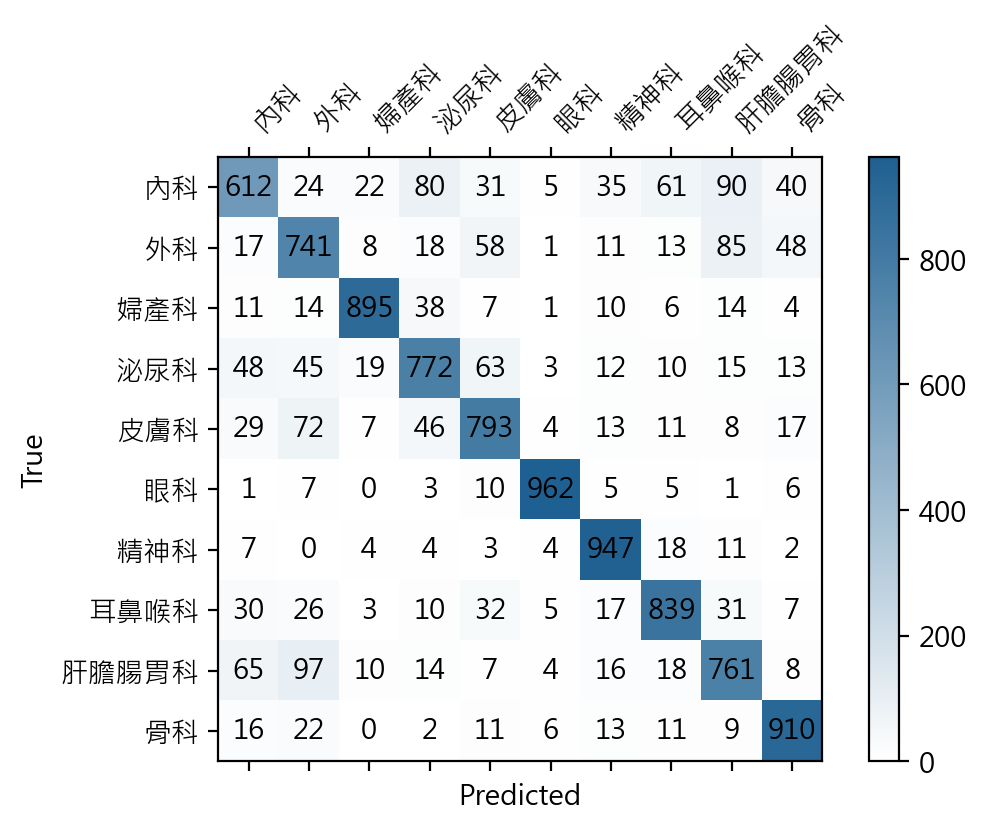
\includegraphics[width=0.5\linewidth]{img/confusion_matrix.png}
			\caption{範例圖片}
			\label{fig:confusion_matrix}
		\end{figure}
		
		\item 表 \texttt{table}
		
		\begin{table}[H]
			\centering 
			\begin{tabular}{|l|c|r|}
				\hline
				\diagbox{左下}{右上} & col 1 & col 2 \\ \hline
				row 1 & tabular 的參數有 l, r, c 與 | & l, c, r 分別表示靠左、中、右 \\ \hline
				row 2 & | 表示一條水平分割線 & 而內文的 hline 則是水平分割線 \\ \hline
			\end{tabular}
			\caption{資料範例}
			\label{tab:data_example}
		\end{table}
		
		\item 內文連結 \texttt{ref}，例如 \ref{fig:confusion_matrix}
	\end{enumerate}
\chapter{研究方法}

本章節將說明本研究之方法流程，包含分群、黑箱分類模型、局部資料生成與局部代理模型建構，並於最後定義實驗設計與評估指標，以確保結果具可重現性與可比較性。:contentReference[oaicite:1]{index=1}

\section{流程與問題設定}
本研究以高維製程量測特徵 $X \in \mathbb{R}^{N \times p}$ 與二元品質標記 $y \in \{0,1\}^N$ 為基礎，目標為同時達成（1）品質預測（2）局部可解釋性分析。
整體流程如下：
\begin{enumerate}
  \item 資料前處理後取得特徵矩陣 $X$ 與標記 $y$。
  \item 對 $X$ 進行分群，得到群標記 $c \in \{0,1,\dots,C-1\}^N$。
  \item 於各群 $c$ 內訓練黑箱分類器 $f_c(\cdot)$，輸出機率 $\hat{p}_c(x)=P(y=1\mid x,c)$。
  \item 於各群內挑選 $\hat{p}_c(x)\approx 0.5$ 的代表點集合，定義局部中心點 $x_0$。
  \item 以 lattice cube 於 $x_0$ 周圍生成局部設計點，並以黑箱輸出作為標記建立局部代理模型 $g(\cdot)$。
  \item 以分類效能與局部擬合指標彙整結果，並進行關鍵案例分析。
\end{enumerate}

\section{分群}
本研究採用分群以處理資料異質性，將原始樣本依特徵空間的結構切分為多個子群，使後續黑箱模型可在群內學習較一致的決策邊界。
令分群演算法輸出 $c_i$ 為第 $i$ 筆樣本之群標記，並以 $X_c=\{x_i: c_i=c\}$ 表示第 $c$ 群之樣本集合。
（本節放置：分群演算法、群數選擇準則、以及群內樣本分佈摘要。）

\section{黑箱模型}
本研究使用梯度提升樹模型作為黑箱分類器，於各群內分別訓練以捕捉非線性關係；黑箱模型輸出為類別機率，用於後續局部代理模型的近似目標。:contentReference[oaicite:2]{index=2}
黑箱模型於第 $c$ 群定義為 $f_c:\mathbb{R}^p \rightarrow [0,1]$，其輸出
\[
\hat{p}_c(x)=f_c(x)=P(y=1\mid x,c)
\]
並以 $\hat{y}=\mathbb{I}(\hat{p}_c(x)\ge t)$ 產生分類結果，其中 $t$ 為分類門檻。

\section{局部擾動（Lattice cube）}
局部代理模型的目的為在 $x_0$ 附近以簡單模型近似黑箱函數。首先於各群內選取黑箱輸出接近 $0.5$ 的樣本集合 $\mathcal{I}_0=\{i:\hat{p}_c(x_i)\approx 0.5\}$，並以其平均作為中心點
\[
x_0=\frac{1}{|\mathcal{I}_0|}\sum_{i\in\mathcal{I}_0} x_i.
\]
為避免量綱影響，於標準化空間生成格點。令標準化轉換為 $S(\cdot)$，則 $z_0=S(x_0)$。
給定步長（半徑）$\delta>0$ 與層數 $k\in\mathbb{N}$，定義偏移集合
\[
\mathcal{M}=\{-k,-k+1,\dots,k\}^p,
\]
並生成局部設計點（標準化空間）
\[
z(m)=z_0+\delta m,\quad m\in\mathcal{M}.
\]
再映射回原始空間 $x(m)=S^{-1}(z(m))$，並以黑箱模型計算局部標記
\[
y^{\text{bb}}(m)=\hat{p}_c(x(m)).
\]
當完整格點數 $(2k+1)^p$ 過大時，以抽樣方式自 $\mathcal{M}$ 取子集以控制局部樣本數。

\section{局部模型（Local surrogate）}
以局部設計點之標準化表示 $z(m)$ 作為解釋變數，以黑箱輸出 $y^{\text{bb}}(m)$ 作為反應變數，建立局部線性代理模型
\[
g(z)=\beta_0+\beta^\top z.
\]
係數 $\beta$ 反映在 $x_0$ 鄰域內黑箱輸出對各特徵方向之局部敏感度；同時保留 $z$ 空間係數以避免尺度混淆，並可再依 $S(\cdot)$ 轉回原始尺度進行詮釋。

\section{實驗設計與交叉驗證}
本研究將資料切分為訓練集與測試集，測試集不參與模型訓練；並於訓練集進行 $K$ 折交叉驗證以估計泛化能力，同時固定隨機種子以確保結果可重現。:contentReference[oaicite:3]{index=3}
分群後之評估採「群內交叉驗證」：對每一群 $c$ 的樣本索引集合分別進行分層抽樣交叉驗證，並彙整各群之 out-of-fold（OOF）預測機率與混淆矩陣。

\section{評估指標}
本研究評估分為兩類：黑箱分類效能與局部代理擬合品質。

\subsection{黑箱分類效能}
以混淆矩陣（TN, FP, FN, TP）彙整分類結果，並計算 Accuracy、Precision、Recall、F1-score，以及以機率輸出計算 ROC-AUC。
此外同時呈現整體 OOF 與各群 OOF 的混淆矩陣，以比較分群前後及群間差異。

\subsection{局部代理擬合品質}
以局部資料 $(z(m),y^{\text{bb}}(m))$ 評估代理模型對黑箱輸出的近似程度，指標包含 $R^2$、Adjusted $R^2$、AIC、BIC 與 SSE。
當不同 $(k,\delta)$ 或局部樣本數設定改變時，以相同指標比較局部近似的穩定性。



	\chapter{研究結果}
	
	\section{分群結果}
	\section{黑箱預測}
	\section{關鍵案例分析}
	\section{討論與限制}


	\chapter{結論}
	
	\section{總結}
	\section{未來工作}
	
	% 引用
	\bibliographystyle{astats}
	\bibliography{references}
	
\end{document}